\begin{figure}[H]
    \centering
    \resizebox{0.95\textwidth}{!}{%
    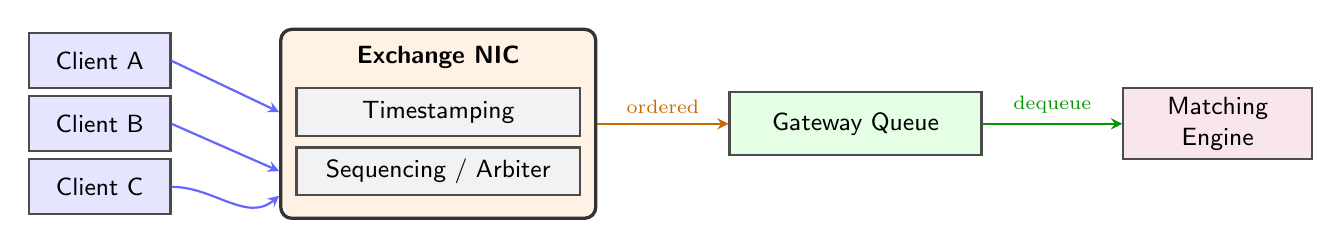
\begin{tikzpicture}[
        font=\sffamily\small,
        client/.style={
            rectangle, draw=black!70, thick,
            fill=blue!10, minimum width=1.8cm,
            minimum height=0.7cm, align=center
        },
        box/.style={
            rectangle, draw=black!70, thick,
            fill=gray!10, minimum width=3.2cm,
            minimum height=0.8cm, align=center
        },
        nicbox/.style={
            rectangle, draw=black!80, very thick,
            fill=orange!10, minimum width=4.0cm,
            minimum height=2.4cm, align=center,
            rounded corners=4pt
        },
        queue/.style={
            rectangle, draw=black!70, thick,
            fill=green!10, minimum width=3.2cm,
            minimum height=0.8cm, align=center
        },
        engine/.style={
            rectangle, draw=black!70, thick,
            fill=purple!10, minimum width=2.4cm,
            minimum height=0.8cm, align=center
        },
        arr/.style={->, thick, >=stealth}
    ]

    % Clients on left
    \node[client] (c1) at (0, 1.6)  {Client A};
    \node[client] (c2) at (0, 0.8)  {Client B};
    \node[client] (c3) at (0, 0.0)  {Client C};

    % NIC box
    \node[nicbox] (nic) at (4.3, 0.8) {};
    \node[font=\sffamily\bfseries\small] at (4.3, 1.65) {Exchange NIC};
    \node[box, minimum width=3.6cm, minimum height=0.6cm]
        (ts) at (4.3, 0.95)
        {Timestamping};
    \node[box, minimum width=3.6cm, minimum height=0.6cm]
        (arb) at (4.3, 0.2)
        {Sequencing / Arbiter};

    % Arrows from clients to NIC
    \draw[arr, color=blue!60] (c1.east) -- (nic.west |- ts.west);
    \draw[arr, color=blue!60] (c2.east) -- (nic.west |- arb.west);
    \draw[arr, color=blue!60] (c3.east) to[out=0, in=220] (nic.west |- arb.south);

    % Queue
    \node[queue] (q) at (9.6, 0.8) {Gateway Queue};

    % Arrow from NIC to Queue
    \draw[arr, color=orange!80!black] (nic.east) -- (q.west)
        node[midway, above, font=\scriptsize] {ordered};

    % Matching Engine
    \node[engine] (me) at (14.2, 0.8) {Matching\\Engine};

    % Arrow from Queue to Engine
    \draw[arr, color=green!60!black] (q.east) -- (me.west)
        node[midway, above, font=\scriptsize] {dequeue};

    \end{tikzpicture}%
    }
    \caption{Simplified model of exchange message ingress.
    Packets arrive concurrently from multiple trading clients and
    are serialised by the Exchange NIC, which applies hardware 
    timestamps and passes messages through an arbiter to enforce 
    strict time-priority ordering. 
    The resulting ordered stream is pushed into a Gateway Queue, 
    from which the single Matching Engine thread consumes sequentially.}
    \label{fig:network_funnel}
\end{figure}
